
\documentclass[twocolumn,twoside]{article}


\usepackage{PRIMEarxiv}

\usepackage[utf8]{inputenc} % allow utf-8 input
\usepackage[T1]{fontenc}    % use 8-bit T1 fonts
\usepackage{hyperref}       % hyperlinks

% setup hyperref
\hypersetup{
    colorlinks=true,
    linkcolor=cyan,
    filecolor=magenta,      
    urlcolor=cyan,
    citecolor=red
}

\usepackage{url}            % simple URL typesetting
\usepackage{subcaption}     % subcaptions
\usepackage{booktabs}       % professional-quality tables
\usepackage{amsfonts}       % blackboard math symbols
\usepackage{nicefrac}       % compact symbols for 1/2, etc.
\usepackage{microtype}      % microtypography
\usepackage{lipsum}
\usepackage{fancyhdr}       % header
\usepackage{graphicx}       % graphics
\usepackage{amsmath}        % math
\graphicspath{{media/}}     % organize your images and other figures under media/ folder

%Header
\pagestyle{fancy}
\thispagestyle{empty}
\rhead{ \textit{ }} 

% Update your Headers here
\fancyhead[LO,RE]{Graph Neural Networks For Next Point Of Interest Recommendation}
\fancyhead[LE,RO]{Dario Loi, Elena Muià, Martina Doku} % Firstauthor et al. if more than 2 - must use \documentclass[twoside]{article}




\DeclareMathOperator{\jax}{Jaccard}


  
%% Title
\title{Graph Neural Networks for Next Point Of Interest Recommendation
}

\author{
  Dario Loi\\
  1940849\\
  %% examples of more authors
   \And
  Elena Muià \\
  1938610 \\
  \And
  Martina Doku \\
  1938629\\
  %% \AND
  %% Coauthor \\
  %% Affiliation \\
  %% Address \\
  %% \texttt{email} \\
  %% \And
  %% Coauthor \\
  %% Affiliation \\
  %% Address \\
  %% \texttt{email} \\
  %% \And
  %% Coauthor \\
  %% Affiliation \\
  %% Address \\
  %% \texttt{email} \\
}


\begin{document}

\twocolumn[
  \begin{@twocolumnfalse}
    \maketitle
    \begin{abstract}
      A POI (Point of Interest) recommendation technique essentially exploits users'
      historical check-ins and other multi-modal information such as POI attributes and
      friendship network, to recommend the next set of POIs suitable for a user. A POI
      recommendation technique essentially exploits users' historical check-ins and other
      multimodal information to recommend the next set of POIs suitable for a user. \newline 
    \end{abstract}
  \end{@twocolumnfalse}

]


\section{Introduction}
This work is a re-implementation of the paper "Hierarchical Multi-Task Graph Recurrent Network for Next POI Recommendation" \cite{main_paper}.
The paper proposes a novel Graph Neural Network (GNN) model for the task of
next Point of Interest (POI) recommendation. The model is designed to
capture the complex relationships between users and POIs, and to
leverage the rich information available in the user-POI interaction
graph. The proposed model is evaluated on a real-world dataset and
compared with a state-of-the-art baseline. The experimental results
show that the proposed model outperforms the baseline and
achieves the paper performance.


\section{Data Preprocessing}
\subsection{Dataset}
The dataset used in this work is the Foursquare dataset\cite{foursquare}. It includes
long-term (about 18 months from April 2012 to September 2013) global-scale
check-in data collected from Foursquare. It contains 33,278,683 checkins by
266,909 users on 3,680,126 venues (in 415 cities in 77 countries).
Those 415 cities are the most checked 415 cities by Foursquare users in the world,
each of which contains at least 10K check-ins.
\subsection{Data Preprocessing}
\begin{figure}[ht]
  \centering
  \begin{subfigure}[b]{0.95\linewidth}
    \centering
    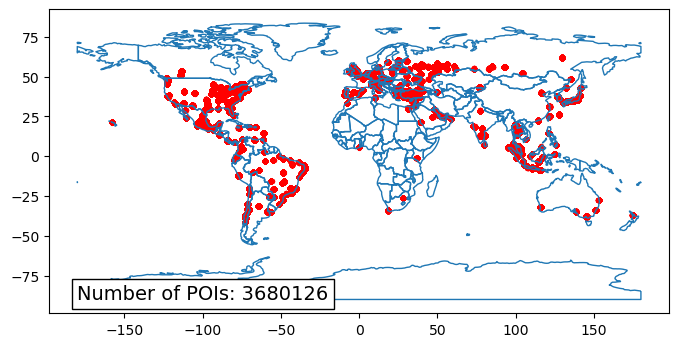
\includegraphics[width=\linewidth]{poi_original.png}
    \caption{Original Points of Interest on the world map}
    \label{fig:data}
  \end{subfigure}
  \hfill
  \begin{subfigure}[b]{0.95\linewidth}
    \centering
    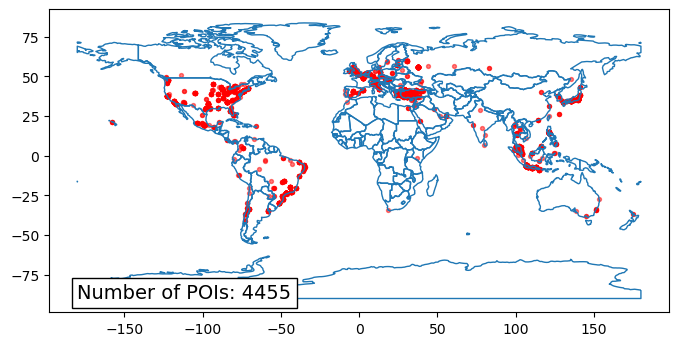
\includegraphics[width=\linewidth]{poi_after_processing.png}
    \caption{Remaining Points of Interest after dataset pruning}
    \label{fig:preprocessed_data}
  \end{subfigure}
  \caption{Comparison of Points of Interest on the world map before (\ref{fig:data}) and after (\ref{fig:preprocessed_data}) preprocessing}
\end{figure}
The dataset is preprocessed to filter out irrelevant data and to prepare
 it for training the models.
The preprocessing follows the same steps as in the original paper, which are:
\begin{itemize}
  \item Filter out users with visit counts less than 20 and more than 50
  \item Remove POIs visited by less than 10 users
  \item Sort the timestamps in chronological order
  \item Divide the data into training and testing sets keeping the first 80\% of the visits for training and the last 20\% for testing
\end{itemize}
The number of POIs before and after processing matches exactly
the numbers reported in the original paper, as shown in Table \ref{tab:poidata}.
\begin{table}
  \caption{Number of POIs}
  \centering
  \begin{tabular}{ll}
    \toprule
    Before Preprocessing & After Preprocessing \\
    \midrule
    \midrule
    $3,680,126$          & $4,455$             \\
    \bottomrule
  \end{tabular}
  \label{tab:poidata}
\end{table}

\subsection{Graph Construction}
The GNN model proposed in the paper leverages two types 
of graphs: spatial and temporal, that have been constructed
as reported in the following sections.
\subsubsection{Spatial Graph}
The spatial graph encodes the relationships between
different points of interest. It is constructed based on the
physical or functional proximity of POIs, by considering
the geo-hash codes of the POIs. The adjacency matrix for the
spatial graph is constructed as follows:
\begin{equation}
  a_{ij} = \begin{cases}
    1 & \text{if } G@4(i) = G@4(j) \\
    0 & \text{otherwise}
  \end{cases}
\end{equation}
\subsubsection{Temporal Graph}
The temporal graph captures the sequential relationships between
POIs. As done in the original paper,
we divided the week in 56 time slots and assigned each check-in to
the corresponding time slots $v^{slot}$. Then we constructed the adjacency matrix
for the temporal graph as follows:
\begin{equation}
  a_{ij} = \begin{cases}
    1 & \text{if } \jax(v^{slot}_i, v^{slot}_j) > 0.9 \\
    0 & \text{otherwise}
  \end{cases}
\end{equation}
where $\jax(v^{slot}_i, v^{slot}_j)$ is the Jaccard
similarity between the two time slots:
\begin{equation}
  \jax(v^{slot}_i, v^{slot}_j) = \frac{|v^{slot}_i \cap v^{slot}_j|}{|v^{slot}_i \cup v^{slot}_j|}
\end{equation}

\section{HMT-RN}
The HMT\_RN (Hierarchical Multi\-Task Recurrent Network) is a
neural network architecture designed for multi-task learning. It employs
embedding layers for users, POIs, and different geo-hash levels,
effectively capturing the hierarchical nature of spatial data.

Central to the HMT\_RN is an LSTM (Long Short\-Term Memory) layer,
which processes sequences of embedded data, capturing temporal dependencies.
The output from the LSTM is concatenated with the embeddings
and passed through several linear layers, each responsible
for predicting the next element in different hierarchical
levels (e.g., POI, geo-hash levels 2 through 6). The model
uses a dropout layer to mitigate overfitting and a
criterion based on cross-entropy loss, applied selectively
to handle padded sequences. Additionally,
it incorporates accuracy metrics at various
levels (Top-1, Top-5, Top-10, Top-20)\footnote{Also called Accuracy@K in the paper\cite{main_paper}} and
Mean Reciprocal Rank (MRR) for performance
evaluation.
\section{GRN}
The GRN (Graph Recurrent Network) is an attention\-based model, developed to
leverage both spatial and temporal graph structures for enhanced predictive
capabilities.

At its core, the GRN integrates graph attention mechanisms
with recurrent layers to precisely process and forecast sequential data points.
This amalgamation enables the model to effectively capture the intricate
spatial and temporal relationships inherent in the data.

The model architecture is composed of multiple key components. Firstly, it employs
graph self-attention mechanisms to dynamically weigh the importance of
neighboring data points within both spatial and temporal contexts.
Central to the GRN is an attentional LSTM (Long Short-Term Memory) layer,
designed to handle sequences of embedded data while capturing temporal
dependencies. Furthermore, the GRN incorporates various linear layers
responsible for predicting the next element in the sequence across
different hierarchical levels. These layers enable the model to forecast
outcomes at multiple granularities, ranging from individual points of interest
(POIs) to higher-order spatial structures represented by different geo-hash levels.

As with the previous model, the GRN integrates dropout regularization and uses
cross-entropy loss as the optimization criterion.

\section{Experiments}
The training procedure utilized the PyTorch Lightning framework,
augmented with the WandbLogger for real-time monitoring and logging of
training metrics. The training dataset was split into train and test sets,
with a batch size of $2048$ for the LSTM model and $128$ for the GRN
 and parallel processing enabled across $4$ workers for
data loading efficiency. The GRN model was instantiated with specific
hyperparameters, including a hidden dimension of $1024$ and a dropout rate of $0.9$
as specified in the reference paper. The training process was configured
for a maximum of $200$ epochs and equipped with callbacks for dynamic
adjustment of learning rates, model checkpointing, and early
stopping based on validation loss.

Throughout the training process, careful attention was paid to memory
management and optimization techniques. The experimental setup aimed to
strike a balance between computational efficiency and model performance,
laying the groundwork for robust experimentation and evaluation of the
GRN architecture.

The values of the metrics during the training process are shown in Figures 
\ref{fig:top1}, \ref{fig:top5}, \ref{fig:top10}, \ref{fig:top20}, and \ref{fig:mrr}.
\begin{figure}[ht]
  \centering
  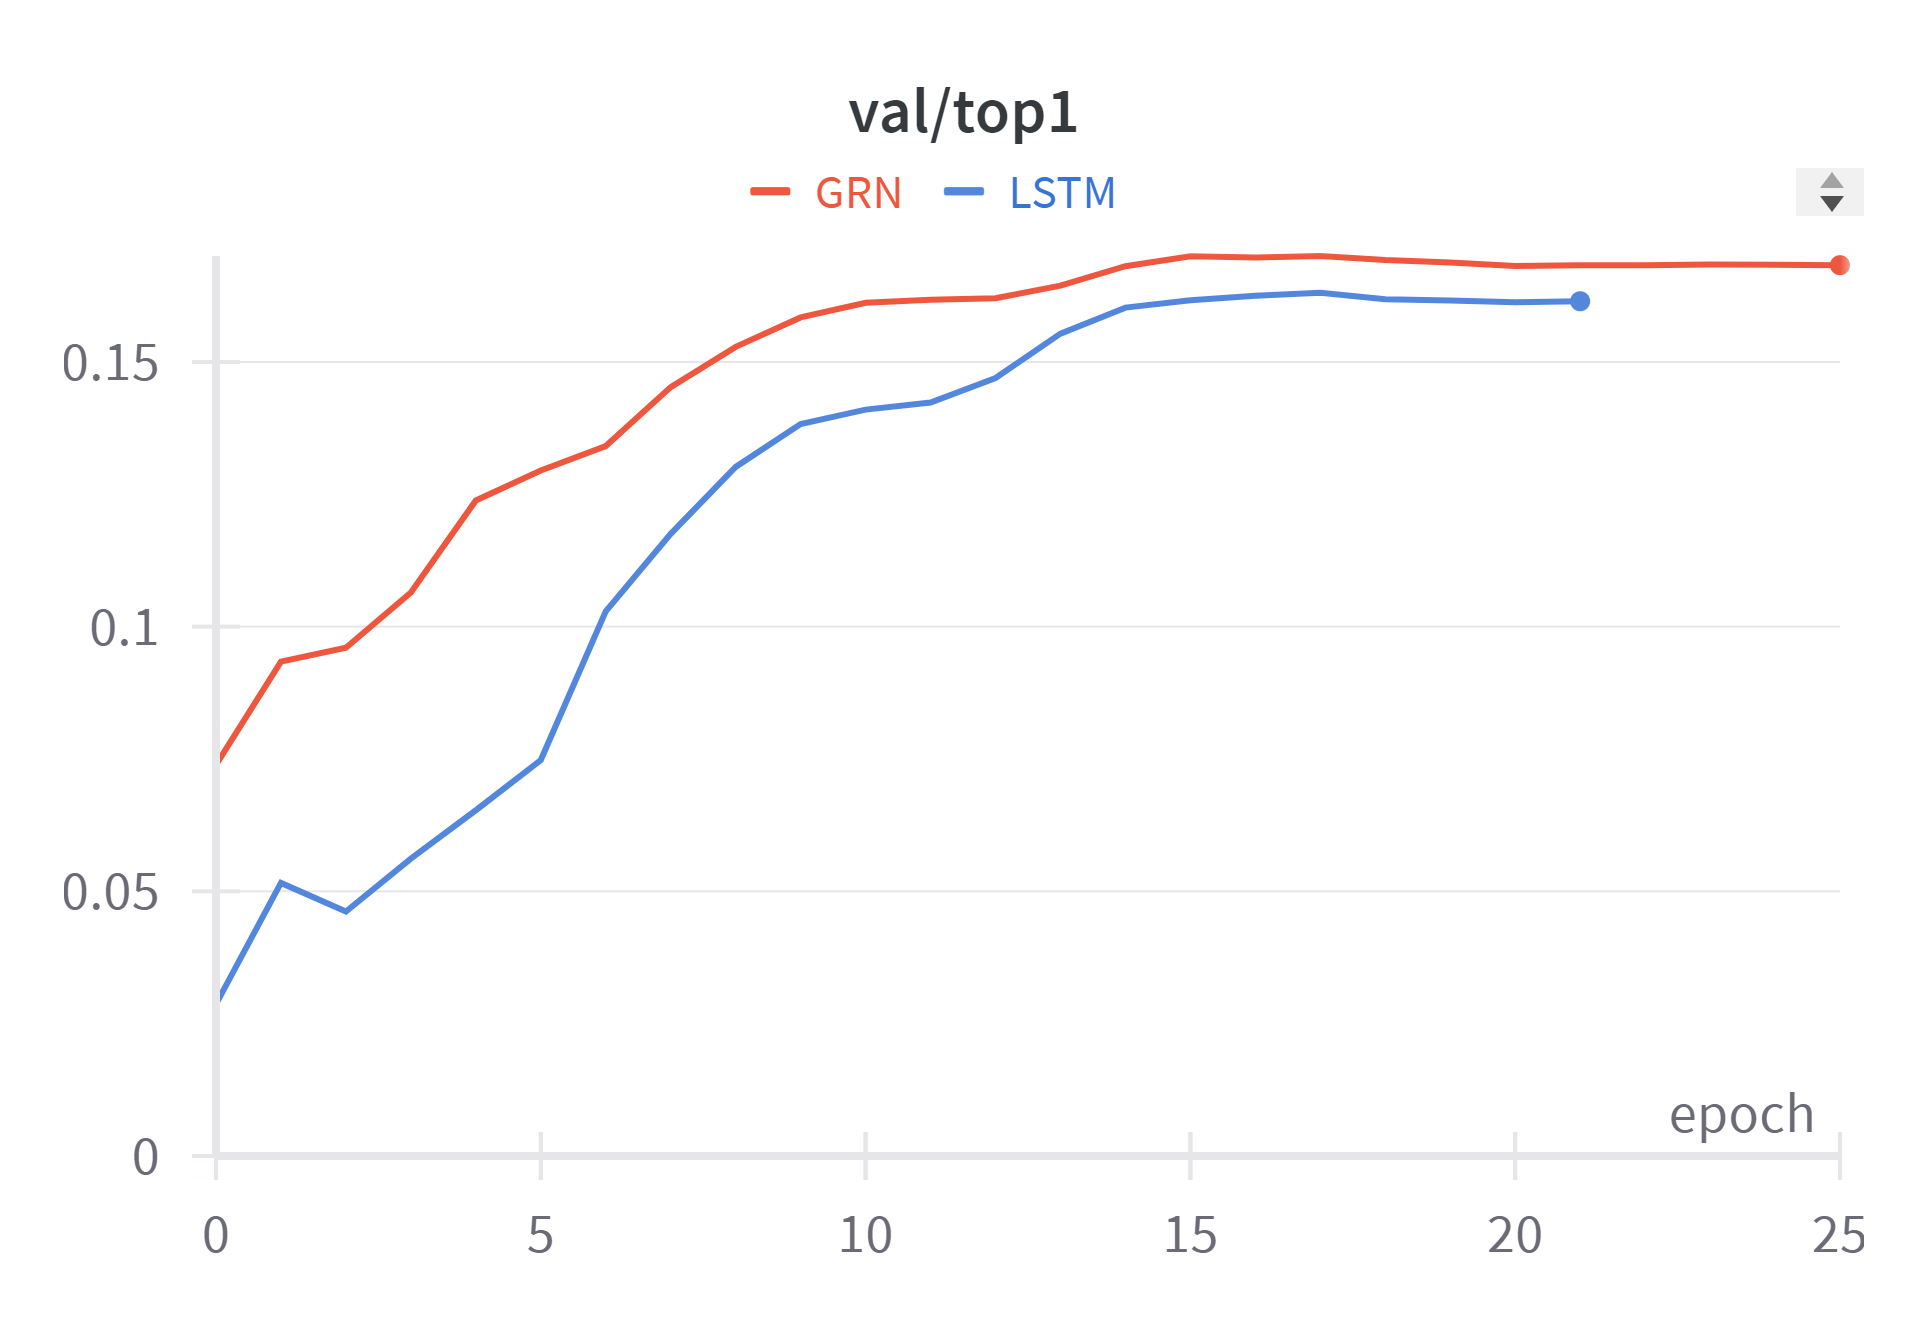
\includegraphics[width=\linewidth]{top1.png}
  \caption{Top-1 accuracy}
  \label{fig:top1}
\end{figure}
\begin{figure}[ht]
  \centering
  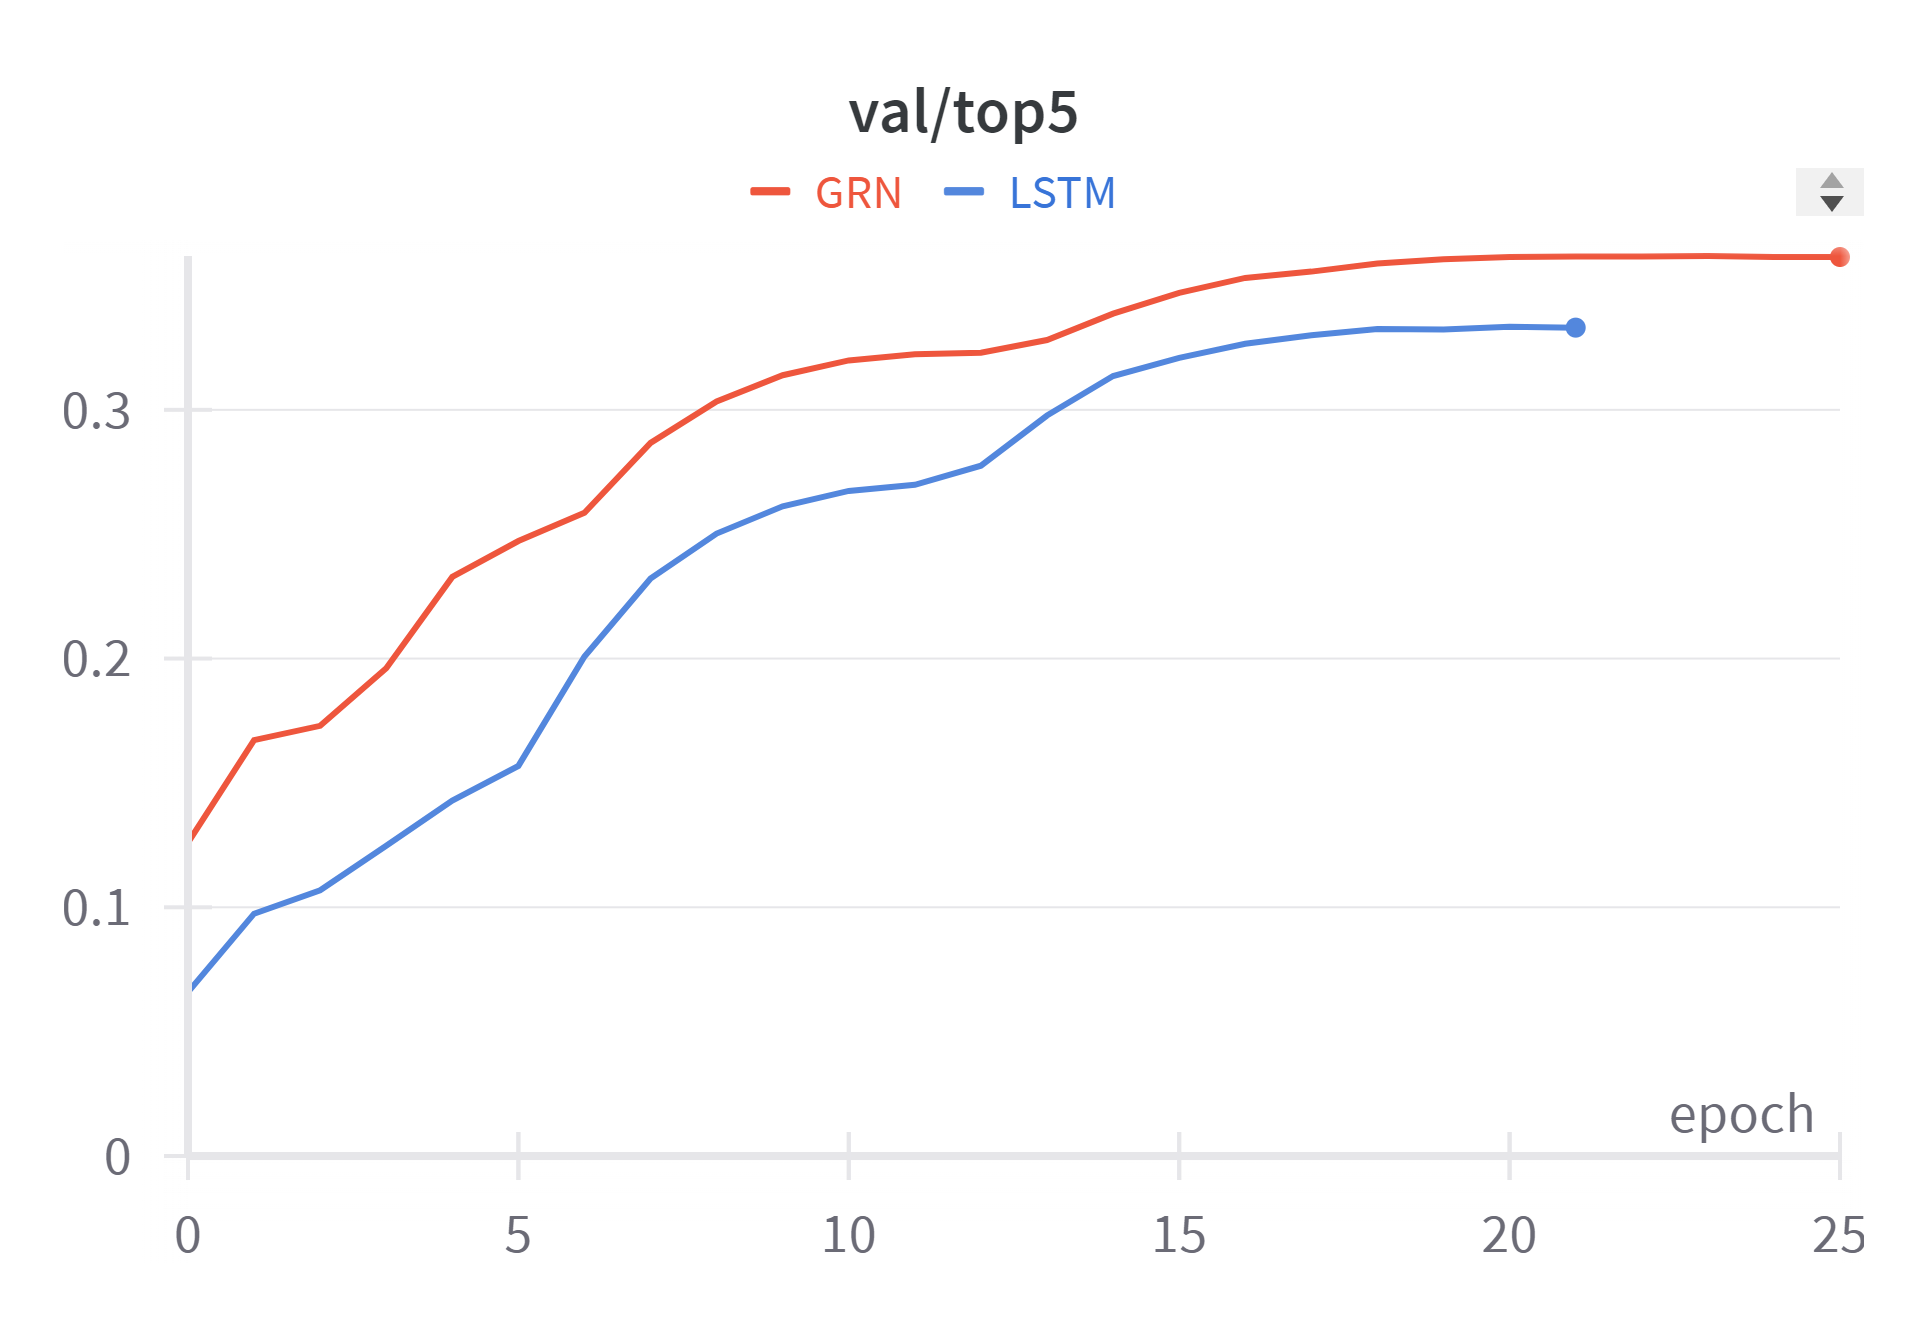
\includegraphics[width=\linewidth]{top5.png}
  \caption{Top-5 accuracy}
  \label{fig:top5}
\end{figure}
\begin{figure}[ht]
  \centering
  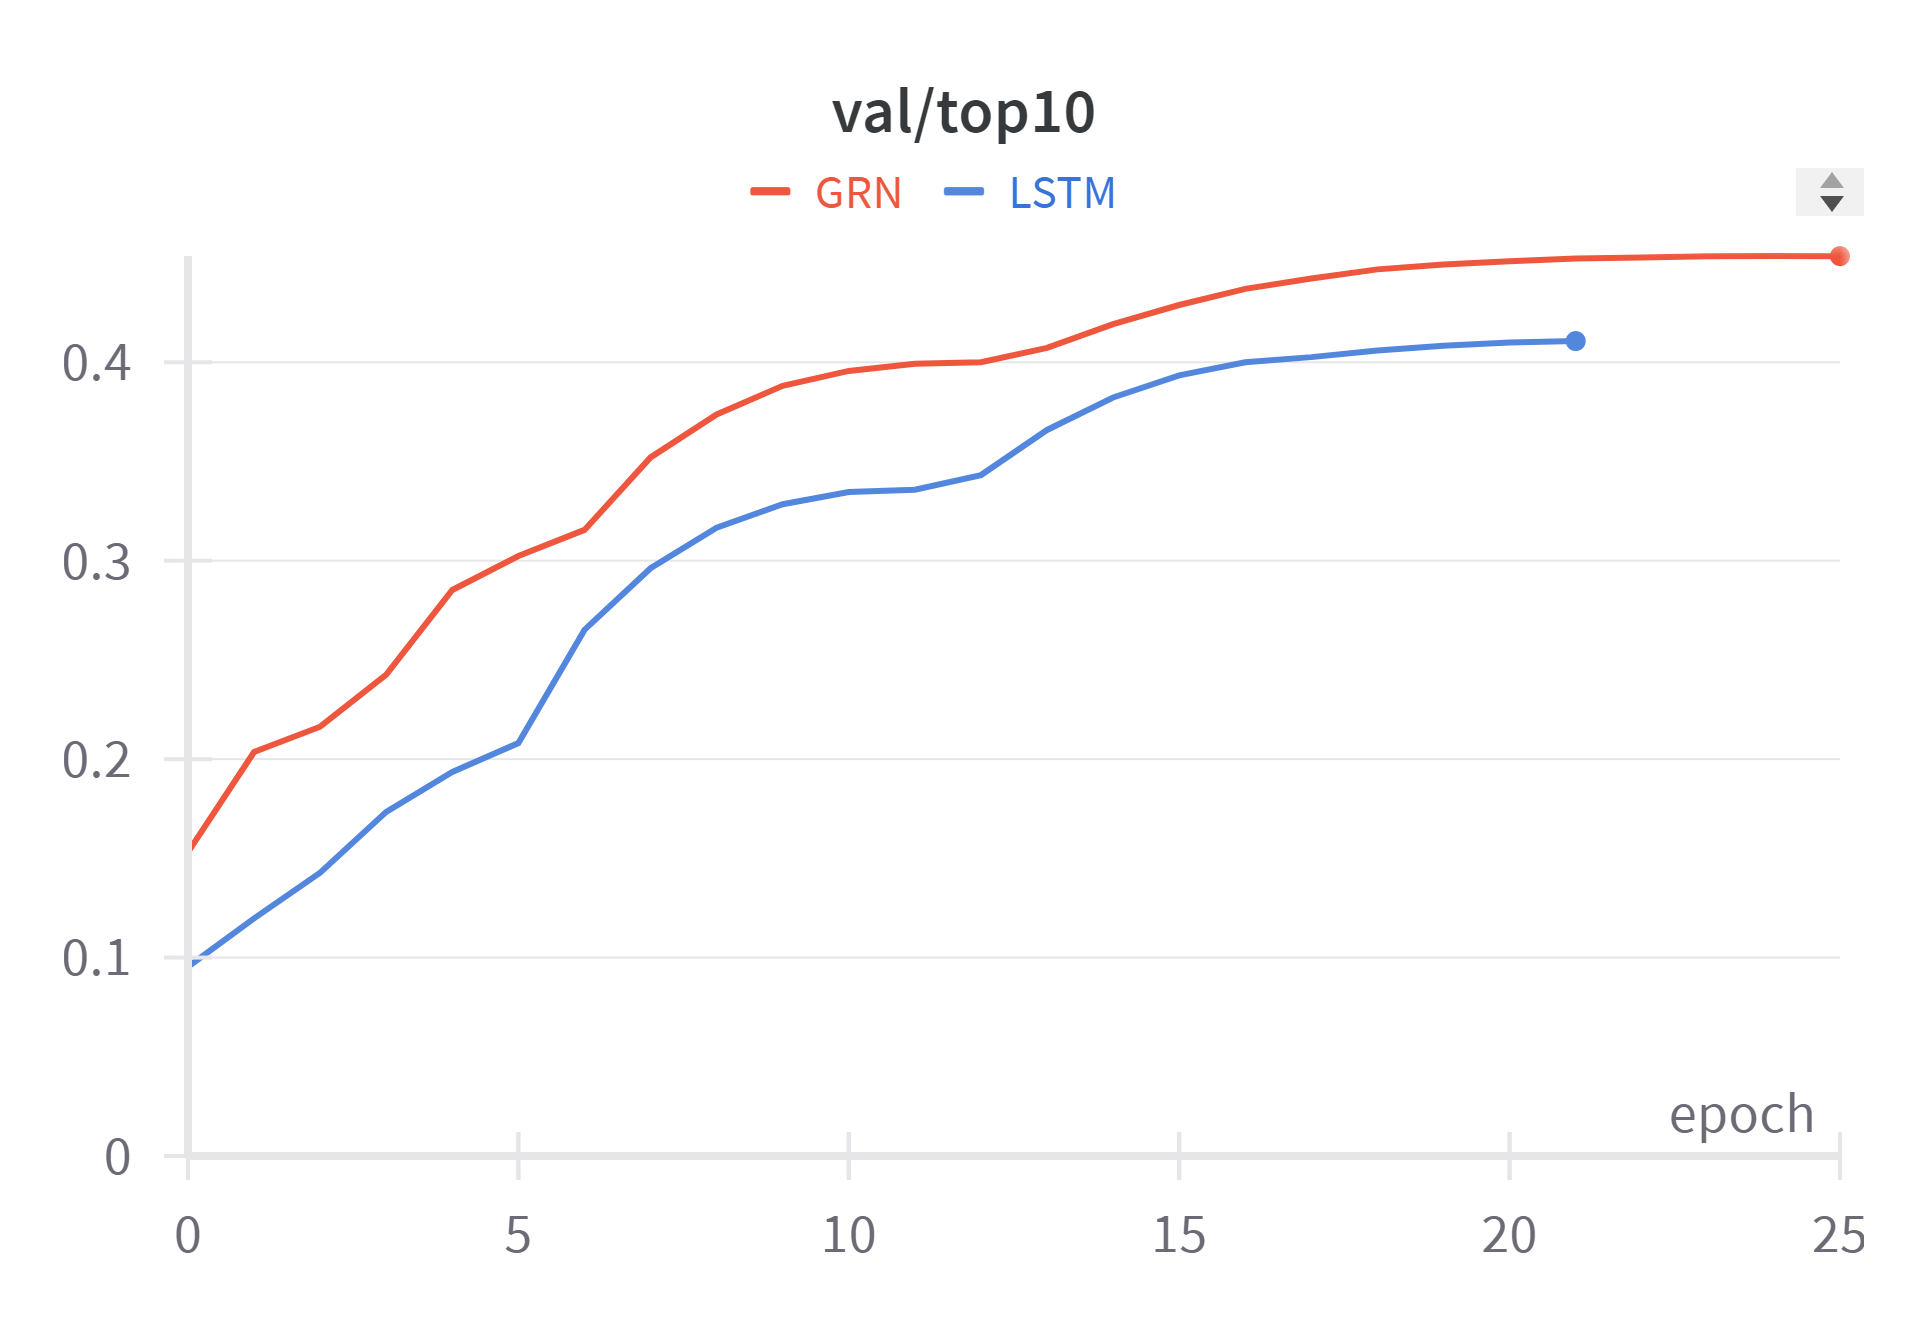
\includegraphics[width=\linewidth]{top10.png}
  \caption{Top-10 accuracy}
  \label{fig:top10}
\end{figure}
\begin{figure}[ht]
  \centering
  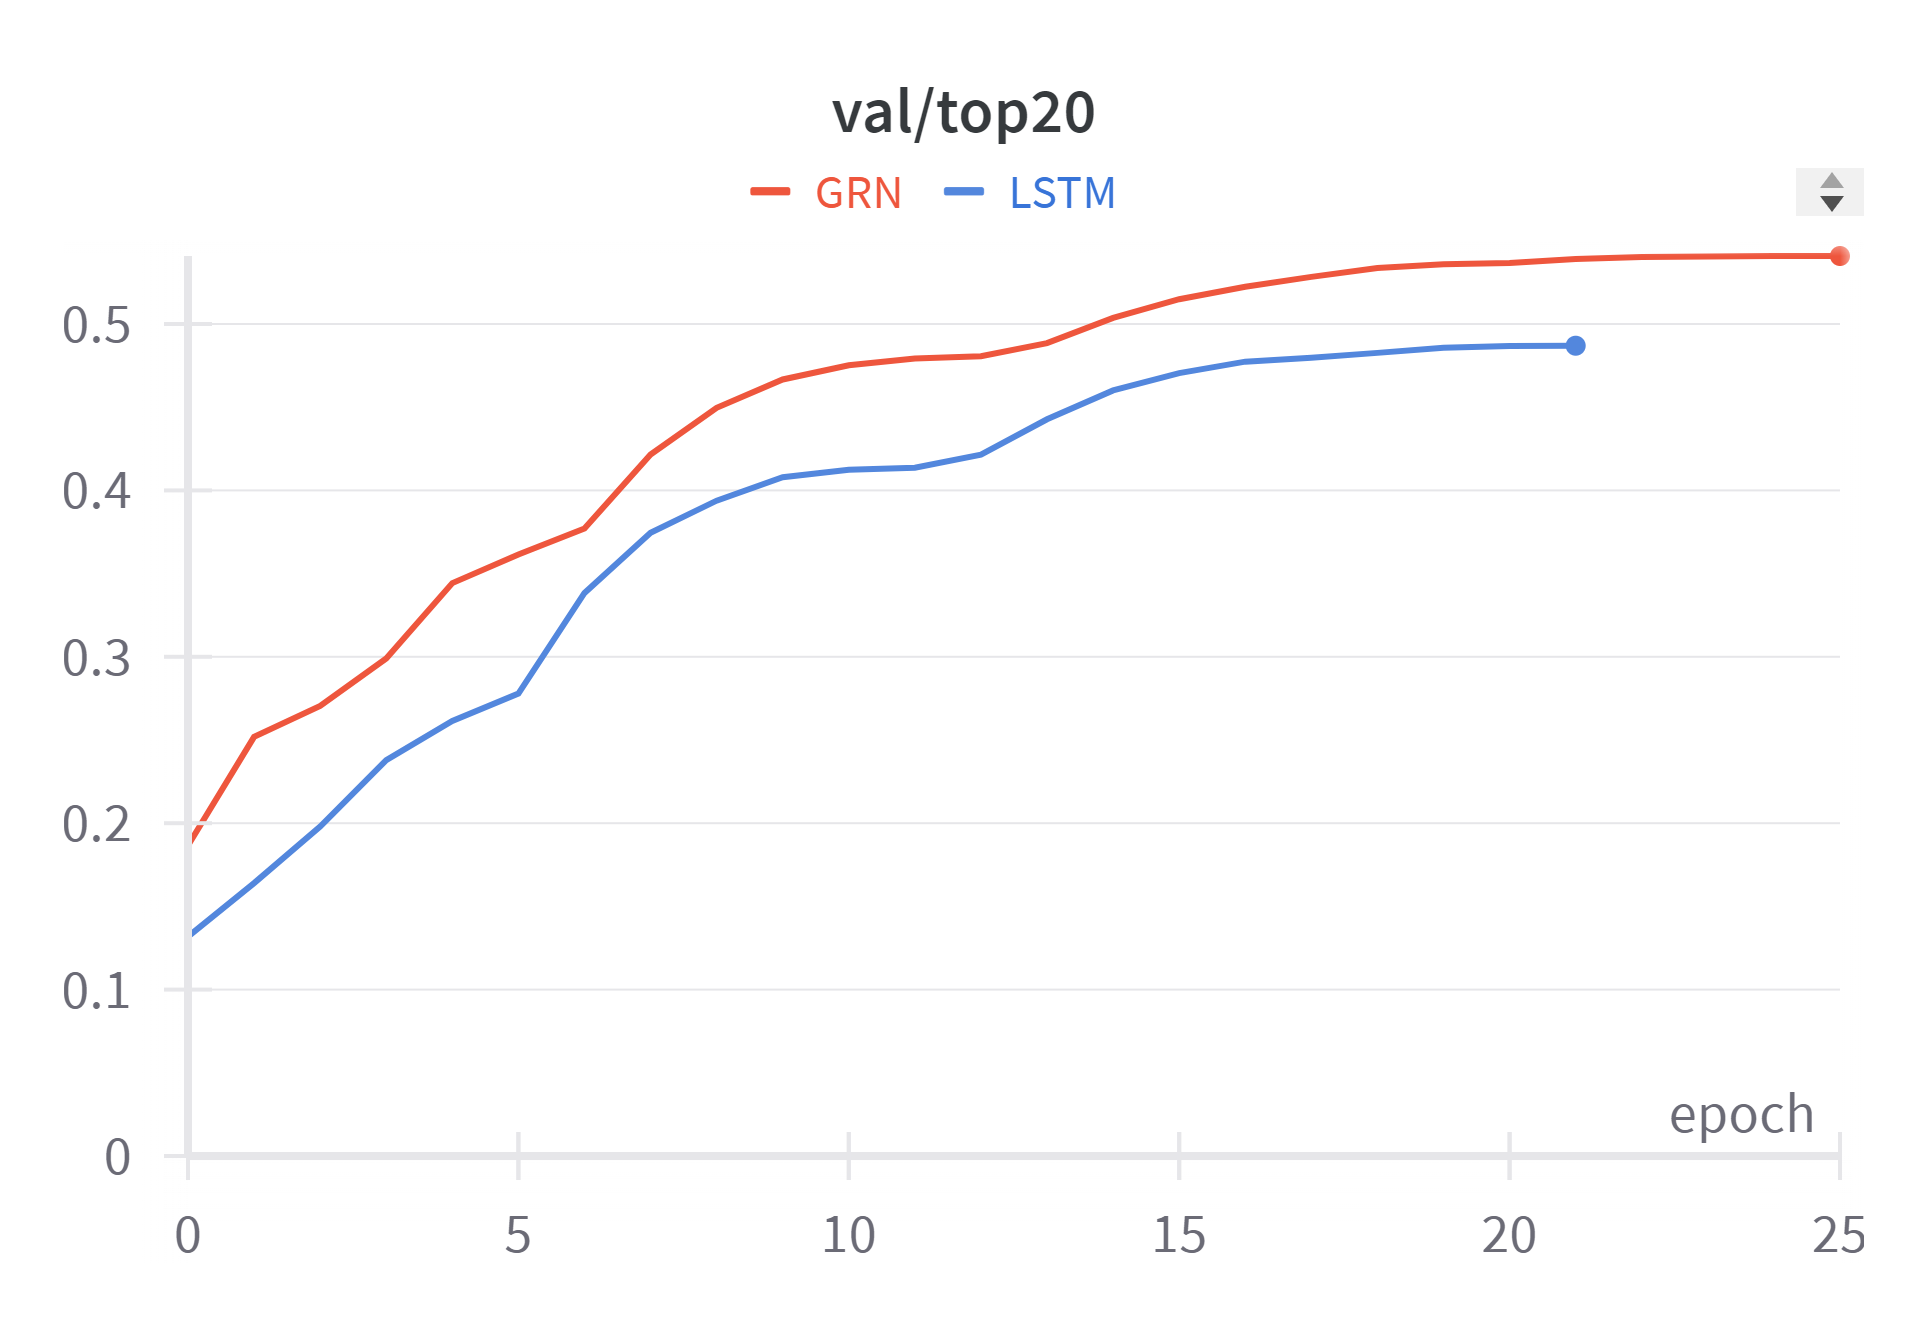
\includegraphics[width=\linewidth]{top20.png}
  \caption{Top-20 accuracy}
  \label{fig:top20}
\end{figure}
\begin{figure}[ht]
  \centering
  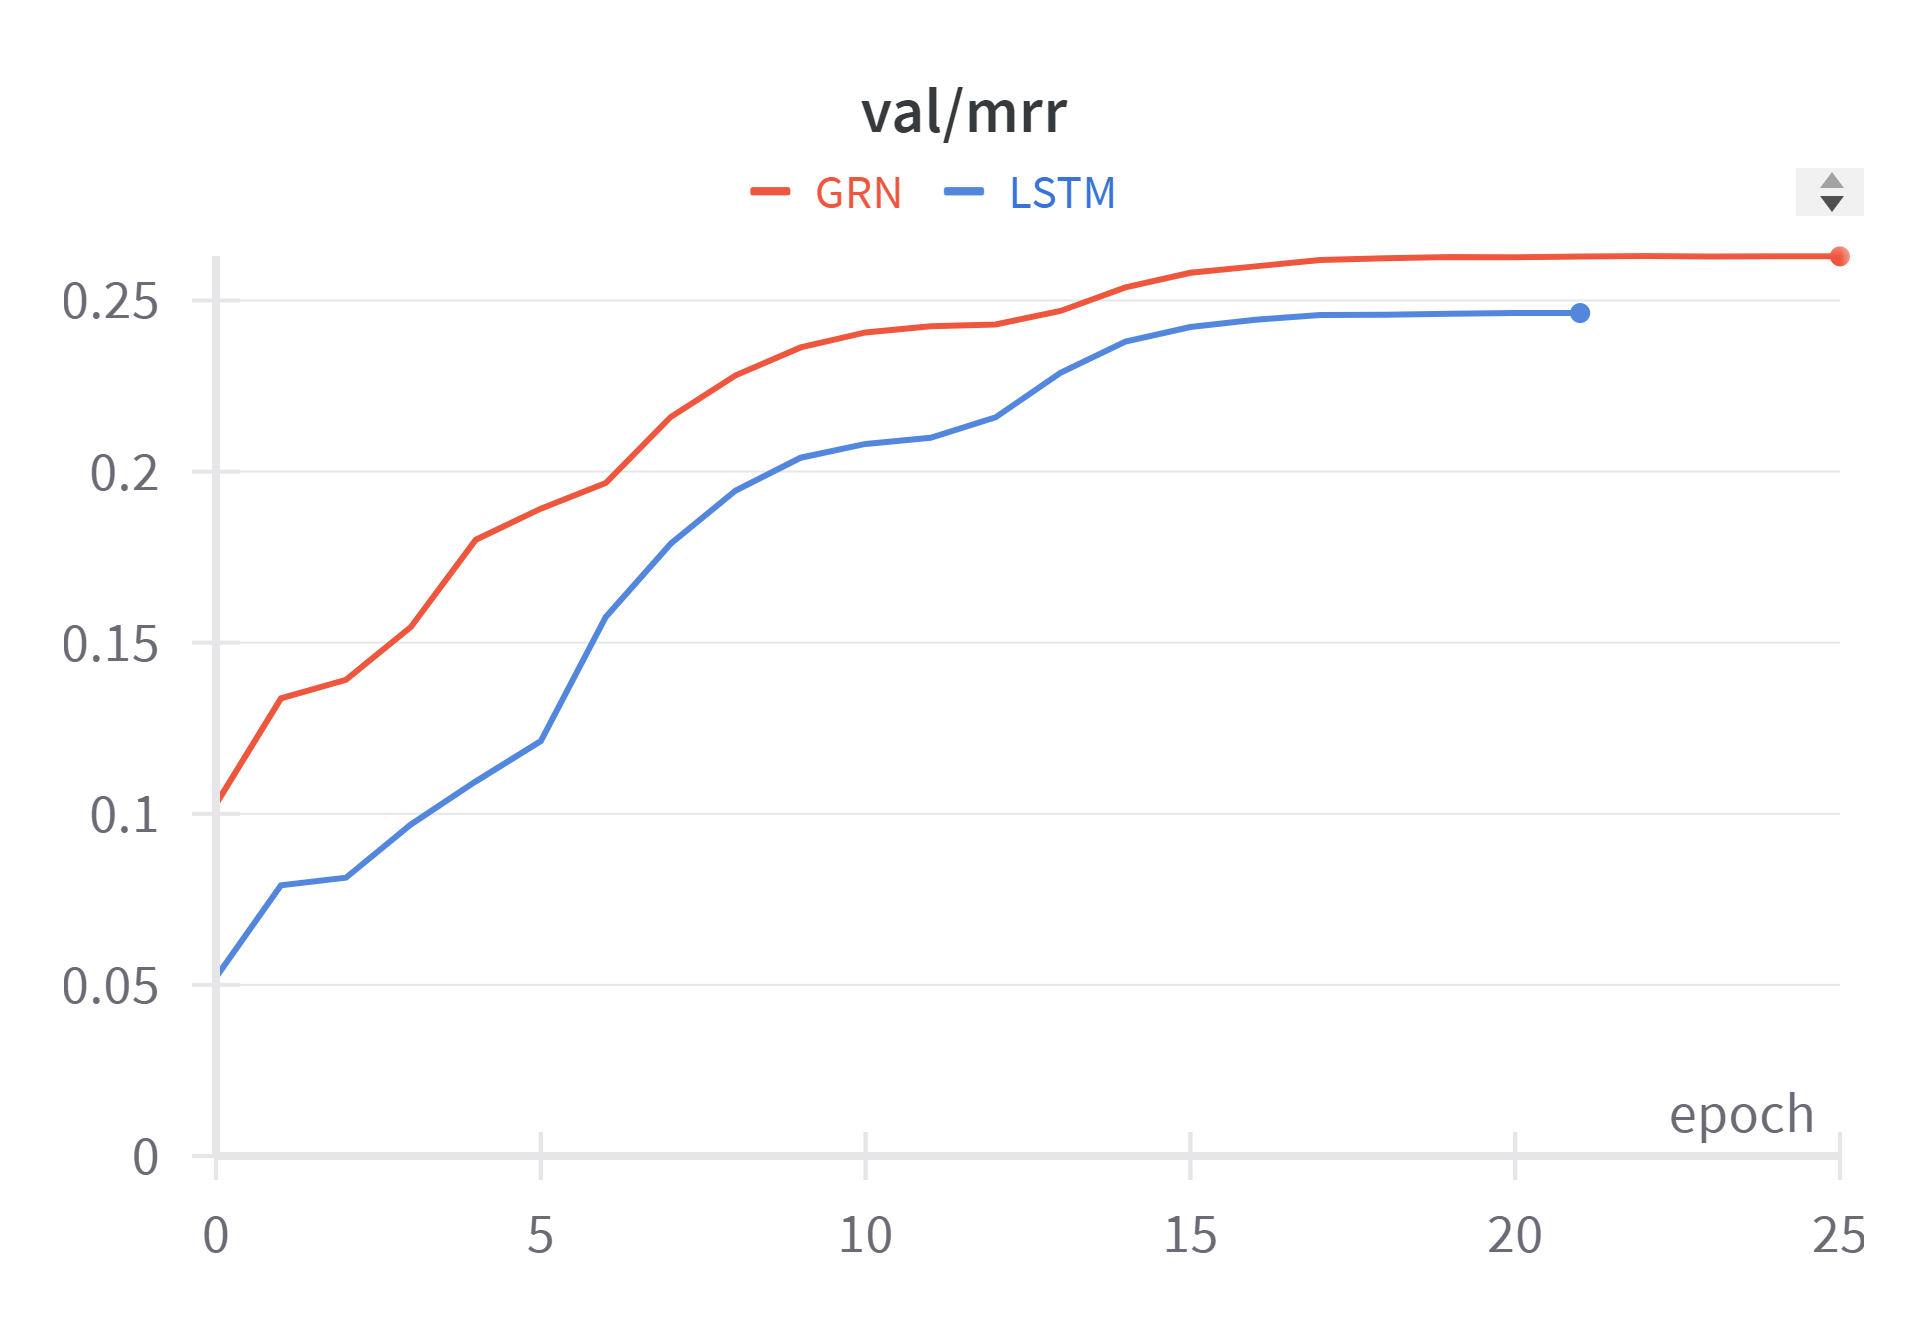
\includegraphics[width=\linewidth]{mrr.png}
  \caption{Mean Reciprocal Rank (MRR)}
  \label{fig:mrr}
\end{figure}


\subsection{Hyperparameters tuning}
In the process of training the Graph Neural Network (GNN) classifier,
 a systematic hyperparameter tuning procedure was employed 
 to optimize the model's performance. Initially,
  the batch size of the classifier was scaled using the power 
  scaling method provided by the \texttt{tuner.scale\_batch\_size} function, 
  which adjusts the batch size to the most appropriate value 
  for efficient training. Following this, the learning rate was
   fine-tuned using a learning rate finder, invoked through the 
   \texttt{tuner.lr\_find} function. This function explored a
    range of learning rates from $5 \times 10^{-5}$ to $1 \times 10^{-3}$ over
     100 training iterations to identify the optimal learning rate
      that minimizes the loss.


\section{Results}
\subsection{Metrics}
The performance of the models is evaluated using the following metrics:
\begin{itemize}
  \item Top-1, Top-5, Top-10, Top-20 accuracy
  \item Mean Reciprocal Rank (MRR)
\end{itemize}
where the top-k accuracy is calculated as follows:
\begin{equation}
  \text{Top-k accuracy} = \frac{1}{N} \sum_{i=1}^{N} \delta(i \in \text{Top-k})
\end{equation}
and the MRR is calculated as follows:
\begin{equation}
  \text{MRR} = \frac{1}{N} \sum_{i=1}^{N} \frac{1}{\text{rank}_i}
\end{equation}
where $\delta$ is the indicator function, $N$ is the number of test samples, Top-k is the set of the k
POIs with the highest predicted scores,
and $\text{rank}_i$ is the rank of the correct POI for the $i$-th test sample.
\subsection{Results}
The results obtained from the experiments are summarized in Table \ref{tab:results}.
The models achieve similar performance to the original paper.
\begin{table}
  \caption{Results}
  \centering
  \begin{tabular}{p{1.55cm}lllll}
    \toprule
    Name & Top-1 & Top-5 & Top-10 & Top-20 & MRR \\
    \midrule
    \midrule
    \textbf{HMT-RN (paper)}\cite{main_paper}\newline & $0.1434$ & $0.2677$ & $0.3213$ & $0.3781$ & $0.2053$ \\
    \textbf{GRN \newline (paper)}\cite{main_paper} & $0.1455$ & $0.2783$ & $0.3394$ & $0.4033$ & $0.2120$ \\
    \midrule
    \midrule
    \textbf{HMT-RN} & \textbf{0.1615} & \textbf{0.3331} & \textbf{0.4107} & \textbf{0.4869} & \textbf{0.2463} \\
    \textbf{GRN} & \textbf{0.1683} & \textbf{0.3615} & \textbf{0.4353} & \textbf{0.5409} & \textbf{0.2629} \\
    \bottomrule
  \end{tabular}
  \label{tab:results}
\end{table}
\section{Conclusion}
We have re-implemented the HMT-RN and GRN models for the task of
next POI recommendation. The models were evaluated on the refence
Foursquare dataset and compared with the original results. The
results show that the models achieve similar performance to the
original paper, demonstrating the effectiveness of the proposed
approach for next POI recommendation.
%References
\begin{thebibliography}{9}
  \bibitem{main_paper}Nicholas Lim, Bryan Hooi, See-Kiong Ng, Yong Liang Goh, Renrong Weng, and Rui Tan. 2022. Hierarchical Multi-Task Graph Recurrent Network for Next POI Recommendation. In Proceedings of the 45th International ACM SIGIR Conference on Research and Development in Information Retrieval (SIGIR '22). Association for Computing Machinery, New York, NY, USA, 1133\-1143. https://doi.org/10.1145/3477495.3531989
  \bibitem{foursquare}Dingqi Yang, Daqing Zhang, Longbiao Chen, and Bingqing Quc. 2015. NationTelescope: Monitoring and Visualizing Large-Scale Collective Behavior in LBSNs.
  Journal of Network and Computer Applications 0, 0 (2015), 1–16.
\end{thebibliography}
\end{document}
